
\section*{Regularization}
    
    So far, we've shown how to make the \textbf{best} model for our \textbf{training data}. But now, we want to move to our \textbf{real} goal: performing well on \textbf{test data}.
    
    This means we want to make a model that is \textbf{general}: it can apply well to \textbf{new data}.
    
    \subsection*{Regularizers}
        
        Only focusing on training data is a \textbf{weakness} for our model - if by chance, we have a training data that doesn't \textbf{match} our overall distribution, we are likely to make a \textbf{bad model}.
        
        \miniex You flip \textbf{4 coins}, and get \textbf{3 heads}. You determine that this coin has a \textbf{75\% chance} of landing heads. It turns out this \textbf{isn't true}: it's a fair coin, and you got \textbf{unlucky}.
        \note{You can also increase sample size (flip more times), but for complex problems this isn't always an option!}
        
         We may need a \textbf{second} way to measure our performance: one that focuses \textbf{less} on \textbf{current} performance, and \textbf{more} on predicting how \textbf{generalizable} it is.
        
        We call this type of function a \textbf{regularizer}.\\
        
        \begin{definition}
            A \vocab{regularizer} is an added term to our \gren{loss function} that helps measure how \purp{general} our hypothesis is.
            
            By \gren{optimizing} with this term, we hope to create a model that works better with \purp{new data}.
            
            This function takes in our \purp{vector of parameters} \gren{$\Theta$} as an input: \purp{$R(\Theta)$}
        \end{definition}
        
        \miniex You figure that the coin is \textbf{equally likely} to bias towards heads or tails: even if it's \textbf{weighted}, you don't know \textbf{which way}. So, you start with \textbf{50-50} odds, and \textbf{adjust} that based on evidence.
        \note{Instead of just focusing on the \textbf{specific} data for our coin, we consider how coins act in \textbf{general}.}
        
    \subsection*{Regularizer for Regression: Prior Knowledge}
        
        Now, the question is, \textbf{how} do we choose our regularizer? What will make our model more \textbf{general}?
        
        We want to \textbf{resist} the effects of random \textbf{chance}, like in the \textbf{coin} example above. In that example, we improved our guess by starting with a \textbf{prior assumption}.
        
        If you have some \textbf{previous} guess, or past experience, you might have some \textbf{model} you \textbf{expect} to work well: the data has to \textbf{convince} you otherwise.
        
        So, we might consider a model \textbf{more different} from that past one, $\Theta_{\text{prior}}$, to be \textbf{suspicious}, and less likely to be good.\\
        
        \begin{concept}
            If we have a \purp{prior} hypothesis $\Theta_{\text{prior}}$ to work with, we might improve our \purp{new} model by encouraging it to be \gren{closer} to the old one.
            
            \begin{equation*}
                R(\Theta)= \norm{ \Theta - \Theta_{\text{prior}} }^2
            \end{equation*}
            
            We measure how \gren{similar} they are using \vocab{square distance}.
            
        \end{concept}
        
        \miniex You have a \textbf{pretty good} model for \textbf{predicting} company profits, but it isn't perfect. You decide to train a \textbf{better} one, but you expect it to be \textbf{similar} to your old one.
        
        
    \subsection*{Regularizer for Regression: No Prior Hypothesis}
    
        But, what if we \textbf{don't have} a prior hypothesis? What if we have \textbf{no clue} what a \textbf{good} solution looks like?
        
        Well, just like in the \textbf{coin} example, we don't expect it to be \textbf{more likely} to be \textbf{weighted} towards heads or tails.
        
        So, even if we \textbf{didn't know} most coins are fair coins, we still would've chosen \textbf{50-50} as our guess.
        
        In this case, as far as we know, every $\theta_k$ term is \textbf{equally likely} to be \textbf{positive or negative} - we have no clue.
        
        So, \textbf{on average}, we could push for it to be \textbf{closer to zero}, so it doesn't drift in any direction too strongly.\\
        
        \begin{kequation}
            In general, our \vocab{regularizer for regression} will be given by \purp{square magnitude} of $\theta$:
            
            \begin{equation*}
                R(\Theta) = \norm{\theta}^2 = \theta \cdot \theta
            \end{equation*}
            
            This approach is called \vocab{Ridge Regression}.
        \end{kequation}
        
        \note{We'll discuss why it's called "ridge" regression once we find our solution.}
        
    \subsection*{Why not include $\theta_0$?}
    
        One thing you might immediately notice is that we used the magnitude of $\theta$ instead of $\Theta$: this omits $\theta_0$. Why would we do that?
        
        We'll show that we need to \textbf{allow} the \textbf{offset} to have whatever value works best, and we shouldn't \textbf{punish} it. 
        \note{For simplicity, we won't do any regularization here: we can make our point without it.}
        
        This is best shown with a \textbf{visual} example. Let's take an example with one input $x_1$. So, we have a \textbf{linear} function: \red{$h(x) = \theta_1x_1+\theta_0$}.
        
        \begin{figure}[H]
        \centering
            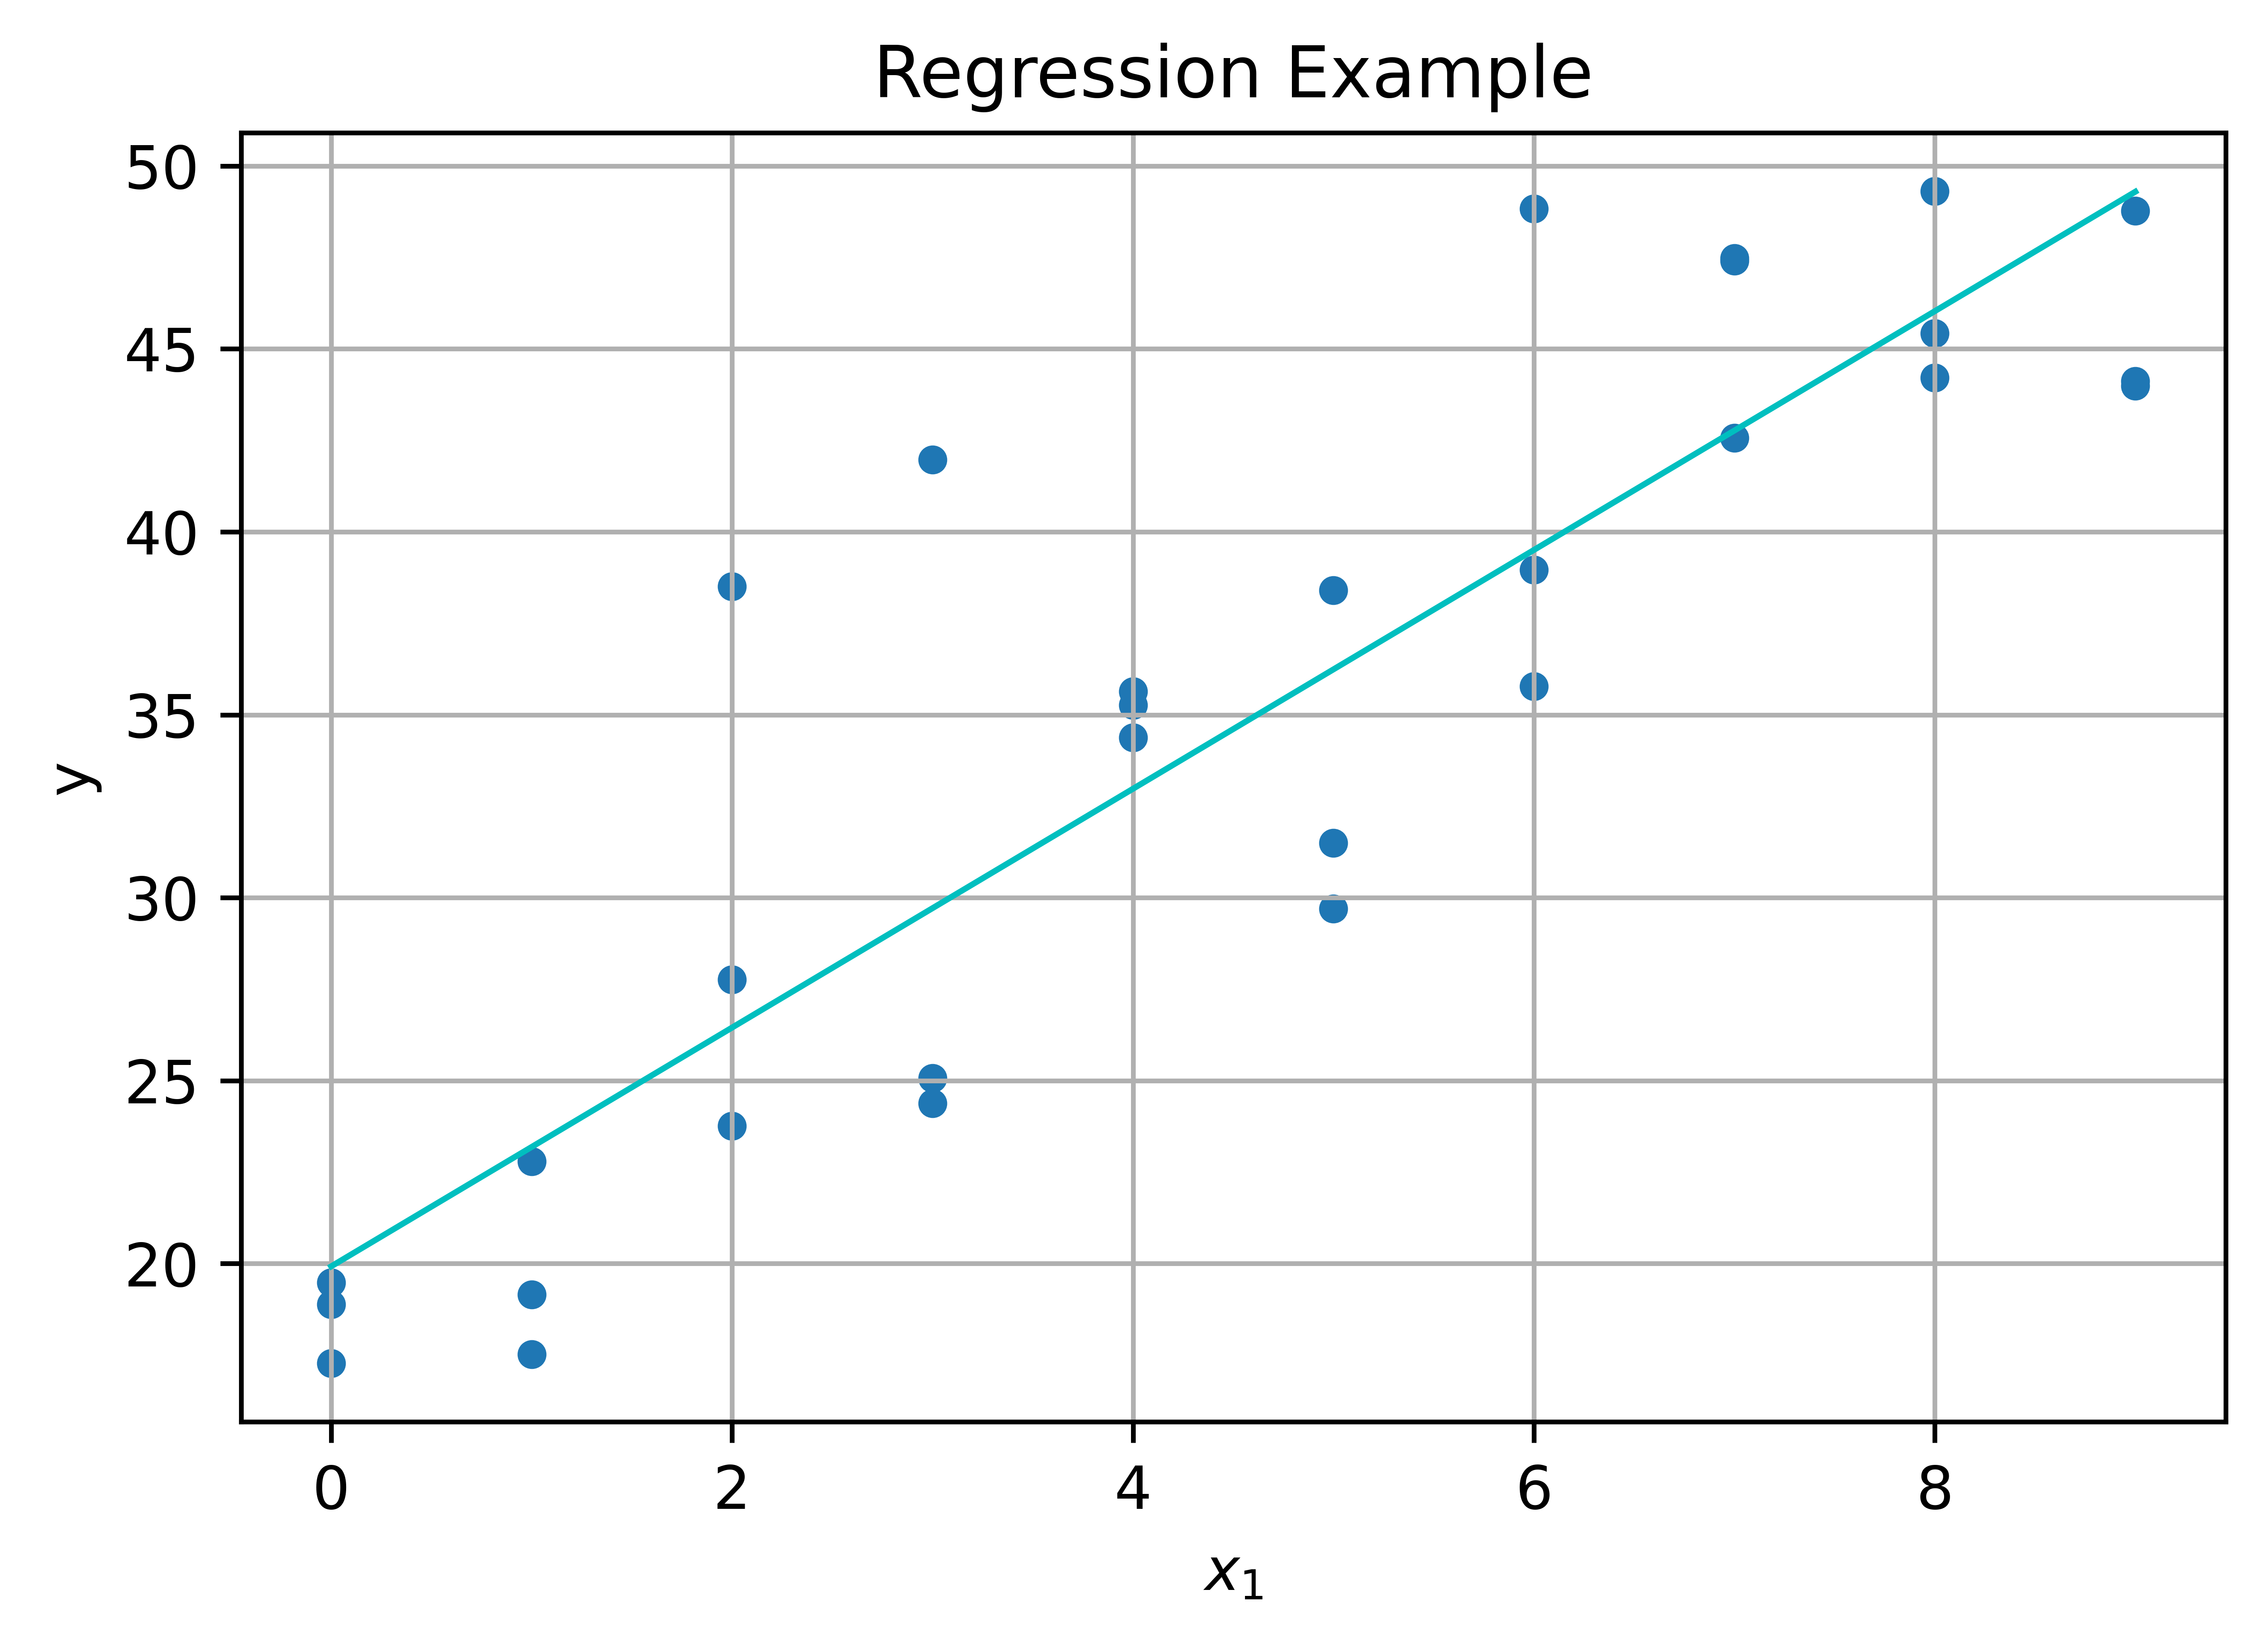
\includegraphics[width=70mm,scale=0.5]{images/regression_images/Regression_Keep_Offset.png}
        
            \caption*{Our regression example.}
        \end{figure}
        
        Let's suppose we \textbf{push} for a \textbf{much lower} (offset) $\theta_0$ term, while keeping everything else the \textbf{same}:
        
        \begin{figure}[H]
        \centering
            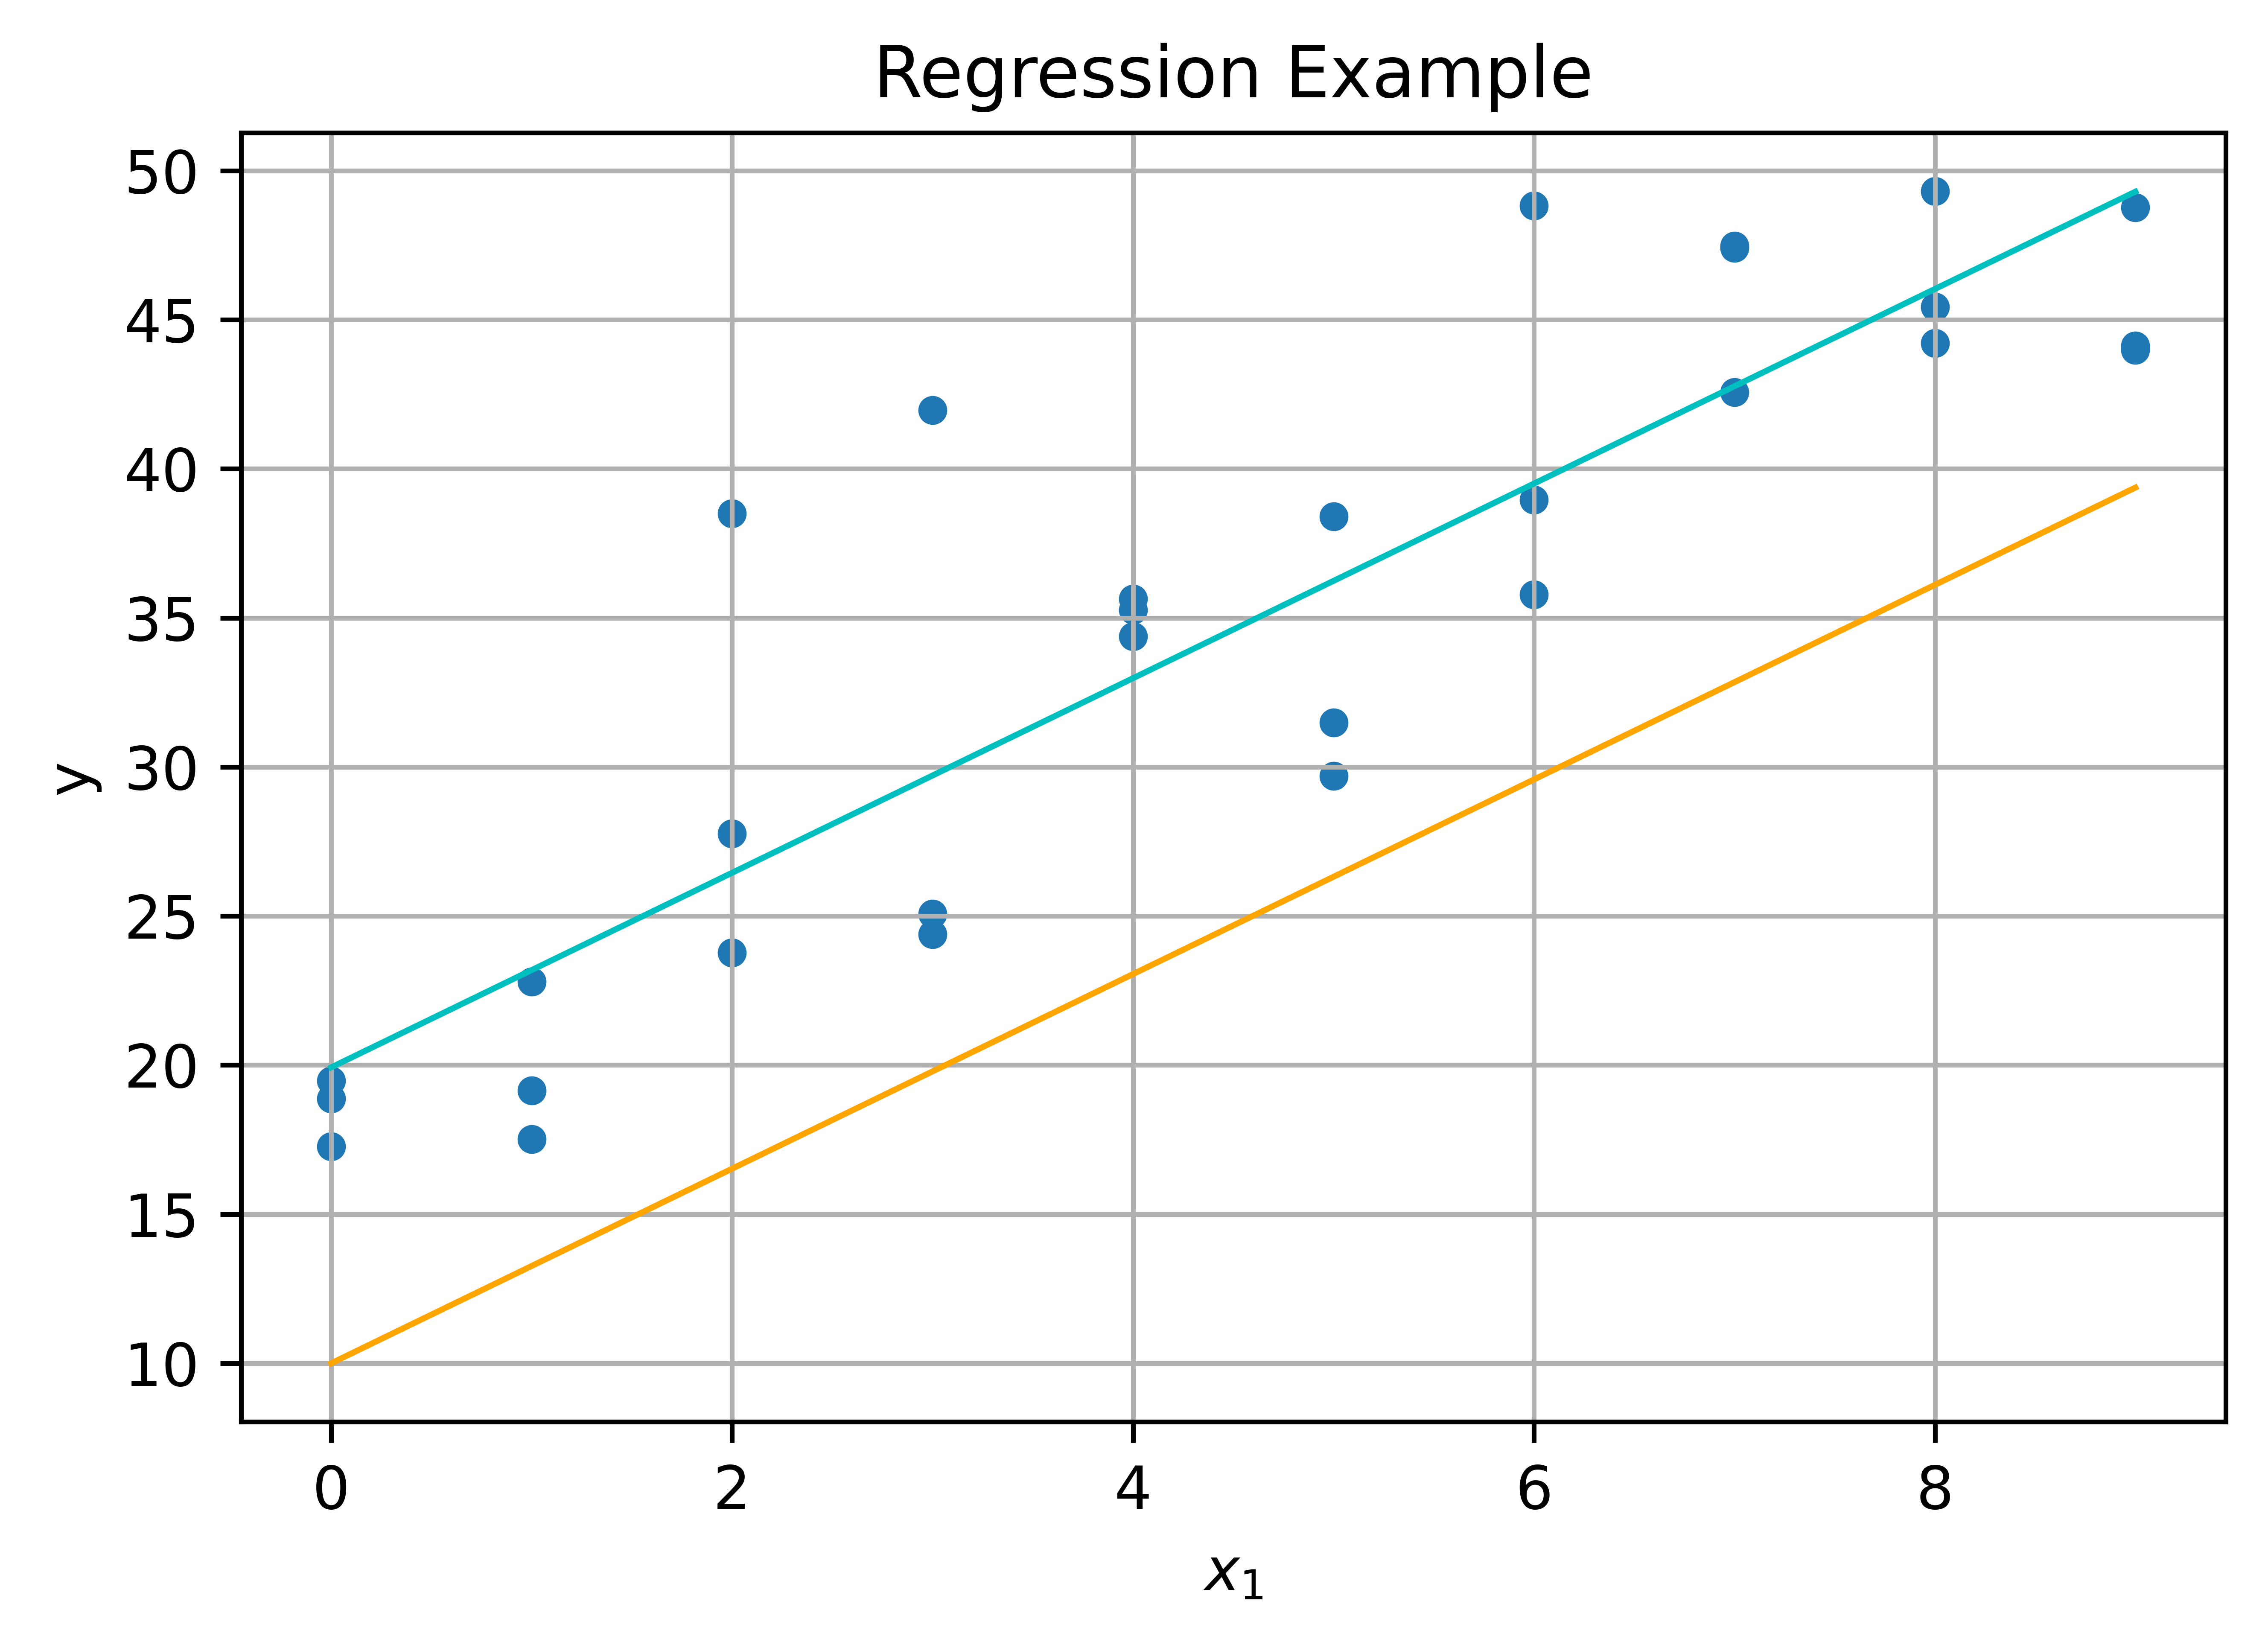
\includegraphics[width=70mm,scale=0.5]{images/regression_images/Regression_Remove_Offset.png}
        
            \caption*{Reducing our offset pulls our line further away from all of our data! That's not helpful.}
        \end{figure}
        \note{And regularizing $\theta_1$ wouldn't make this any better: it would just be flatter.}
        
        This shows that we \textbf{need} our offset! We use it to \textbf{slide} our hyperplane around the space: if all of our data is \textbf{far} from $(0,0)$, we need to be able to \textbf{move} our \textbf{entire line}.
        
        So, we'll keep $\theta_0$ \textbf{separate} and \textbf{allow} it to take whatever value is \textbf{best}.\\
        
        \begin{concept}
            We \purp{do not regularize} our \purp{offset} term, $\theta_0$. 
            
            Instead, we allow $\theta_0$ to \gren{shift} our hyperplane wherever it \gren{needs} to be.
        \end{concept}
        
        The other terms $\theta$ control the \textbf{orientation} of the hyperplane: the \textbf{direction} it is \textbf{facing}. We \textbf{regularize} this to push it towards less "complicated" orientations.
        \note{This will be discussed more in-depth in the Classification chapter!}

        
    \subsection*{A second benefit of regularization}
    
        Another benefit of regularization is that it solves a second problem: having \textbf{multiple optimal solutions}.
        
        If we have \textbf{multiple} best outcomes, we have to pick which one to \textbf{choose}. We can make this choice by \textbf{picking} the one with the \textbf{smallest} magnitude.
        
        We can \textbf{visualize} the problem of "multiple best solutions" a couple different ways:
        
        \begin{figure}[H]
        \centering
            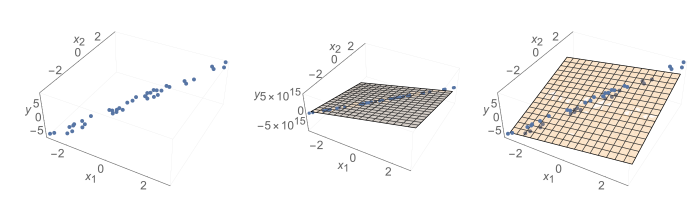
\includegraphics[width=120mm,scale=0.5]{images/regression_images/Regularizer_Multiple_Solutions.png}
        
            \caption*{There are many \textbf{planes} that can go through this line: multiple equally good solutions!}
        \end{figure}
        
        \begin{figure}[H]
        \centering
            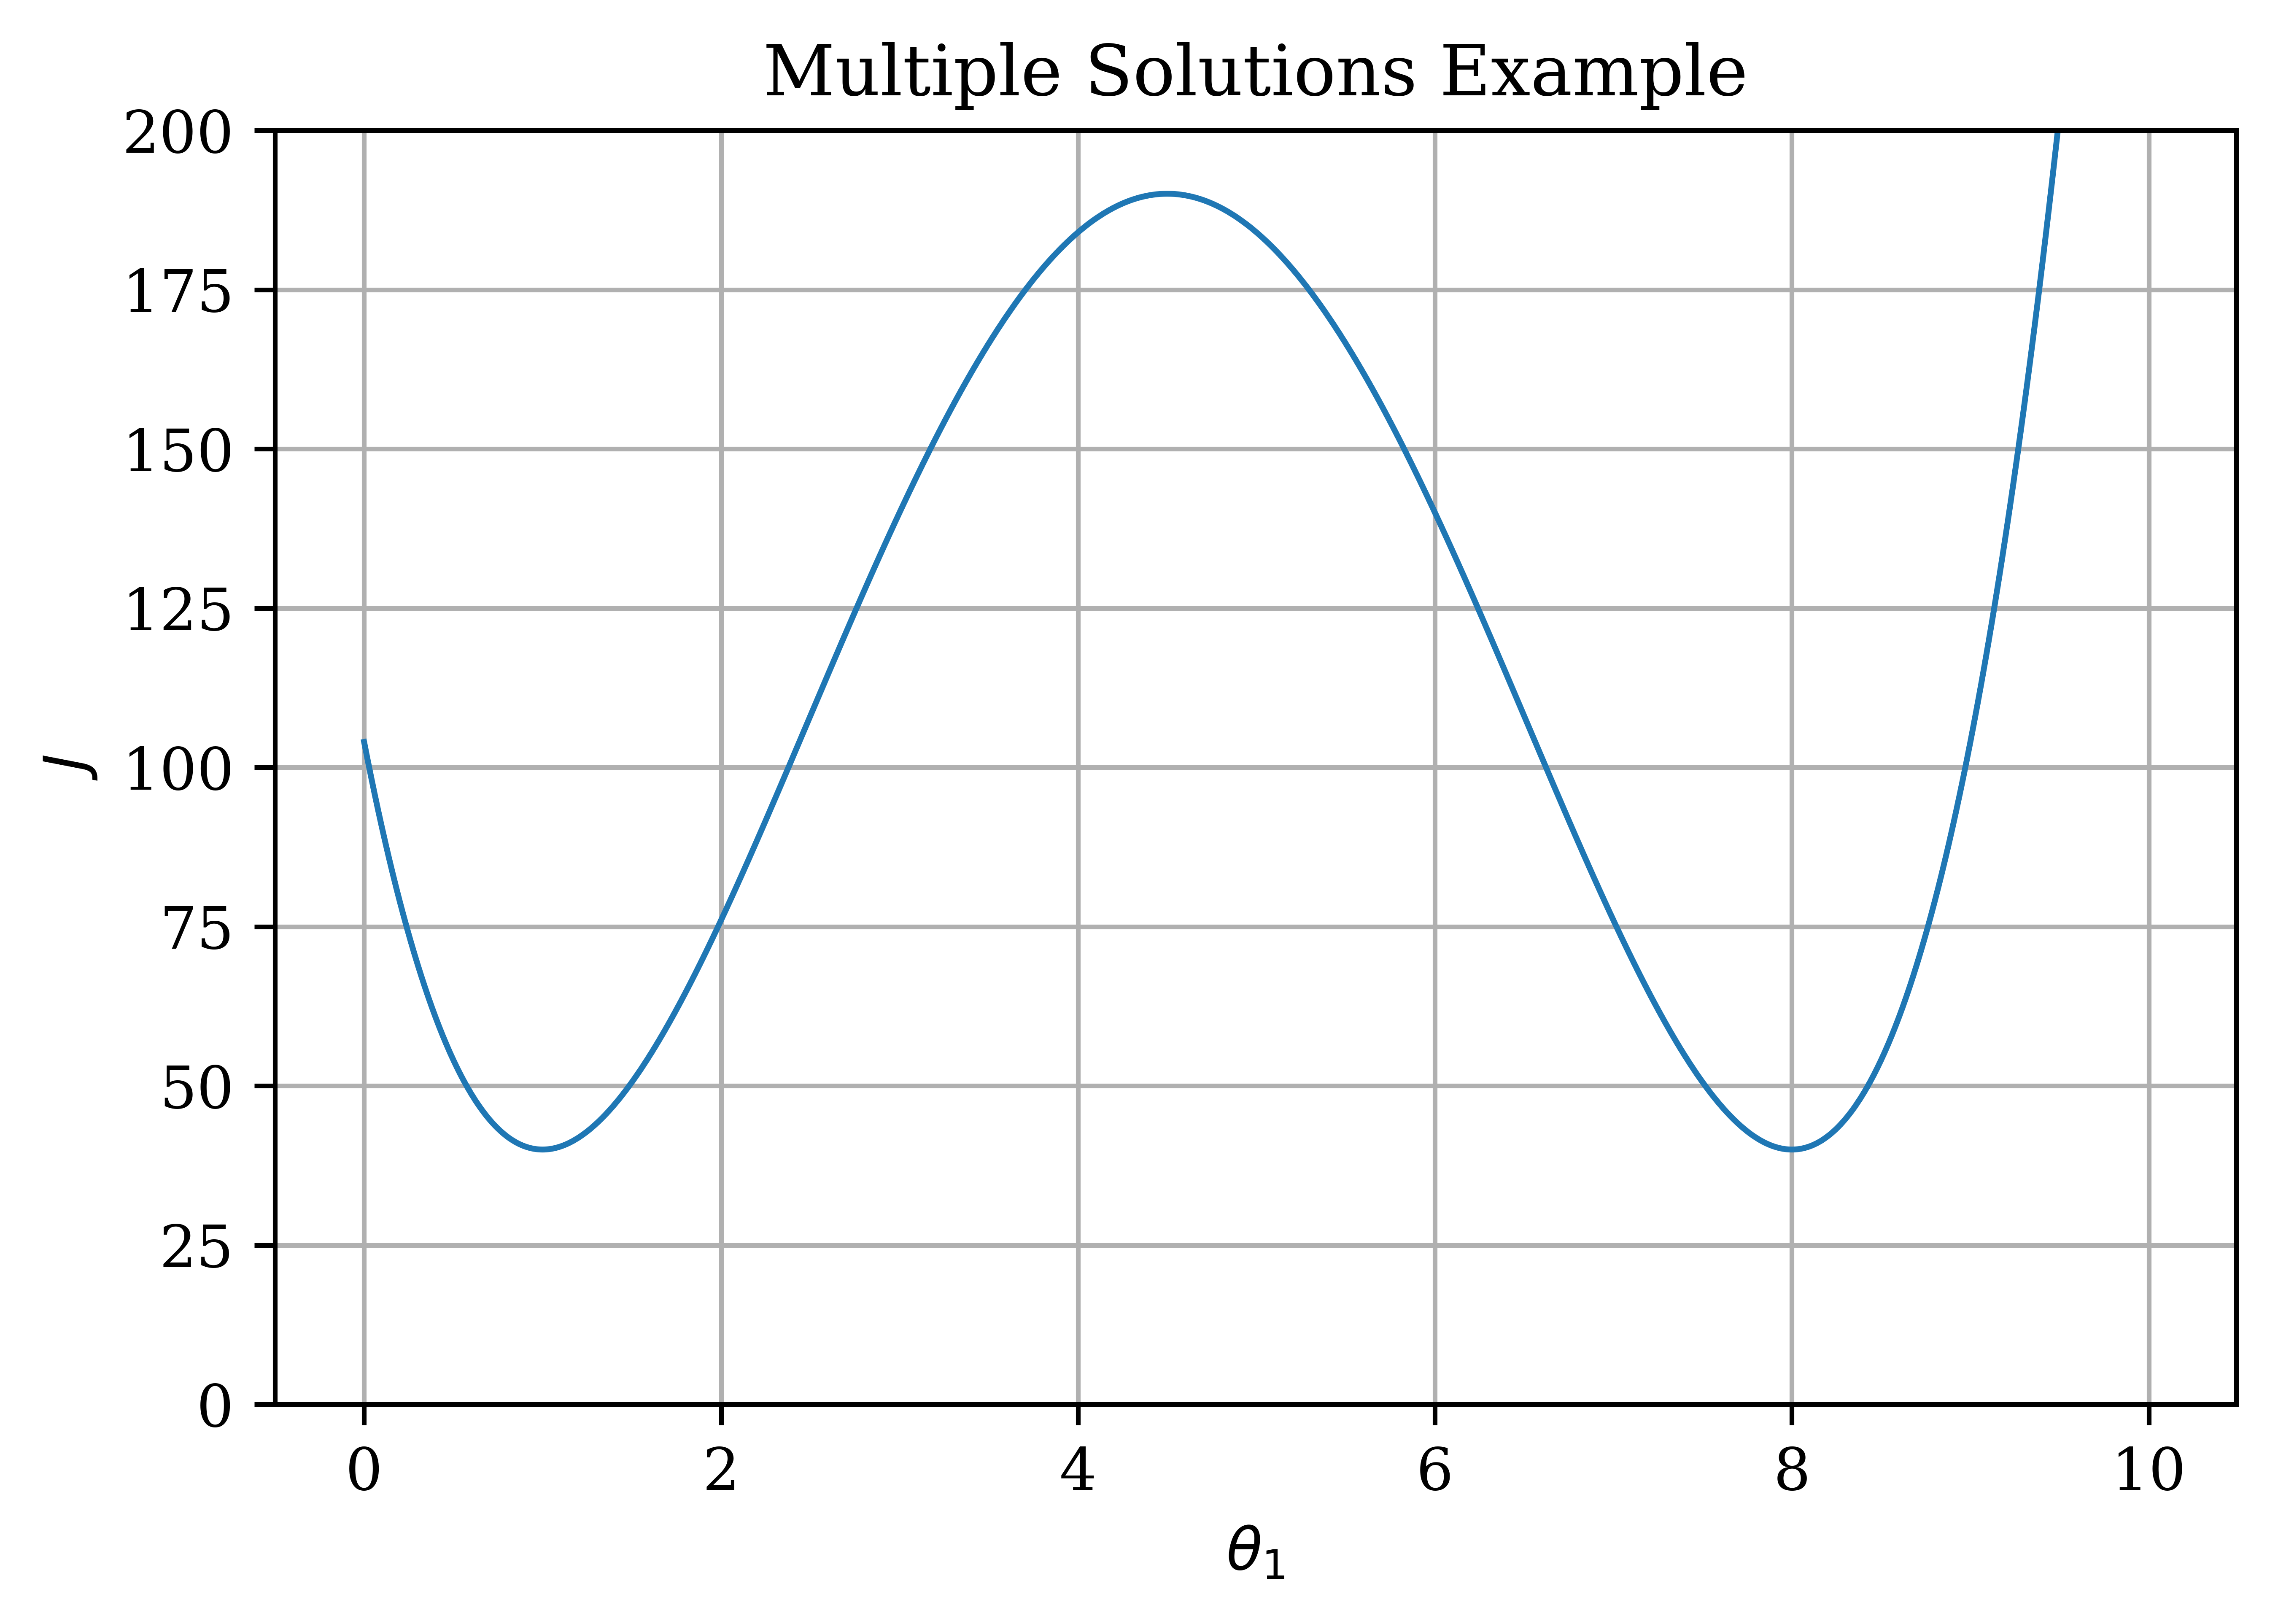
\includegraphics[width=70mm,scale=0.5]{images/regression_images/Regression_Multiple_Solutions_Example.png}
        
            \caption*{This compares different hypotheses ($\theta_1$) and sees how well they perform ($J$): two are equally good!}
        \end{figure}
        
        Either way, we can pick a solution based on lowest $\theta$ \textbf{magnitude}!
        
    \subsection*{A Math Perspective: Unique Solutions}    
        
        We can also view this problem more \textbf{mathematically}.
        
        Let's look at our \textbf{analytical} solution:
        
        \begin{equation}
            \theta = 
                \inv{  \left(  XX^T  \right)  }   X Y^T
        \end{equation}
        
        This solution only works if $\inv{  \left(  XX^T  \right)  }$ is \textbf{valid}. But we have a problem: \textbf{not all matrices} have \textbf{inverses}. 
        
        If $XX^T$ has a \textbf{determinant} of \textbf{zero}, then we cannot find an inverse. 
        \note{This is an important idea in linear algebra! If you don't know what this means, here's a 
        \href{https://www.youtube.com/watch?v=uQhTuRlWMxw&list=PL0-GT3co4r2y2YErbmuJw2L5tW4Ew2O5B&index=8}{great video}.
        }
        
        Without an inverse, we have \textbf{no unique solution}! This is a problem.
        
        This is one thing our \textbf{regularizer} $R(\Theta)$ helps us solve: we'll see that our \textbf{new solution} will not have this problem! 
        
        The reason will be clear in the \textbf{algebra}, but it's \textbf{equivalent} to the reason we discussed the above: we take the best \textbf{models} that are all \textbf{equally good}, and pick the one with \textbf{lowest magnitude}.\\
        
        \begin{concept}
            \vocab{Ridge Regression} helps \purp{improve} our model by
            
            \begin{itemize}
                \item Making our model more \purp{general} and resistant to \gren{overfitting}
                \item Making sure \gren{solutions} are \purp{unique}
                \item Keeping our matrix $XX^T$ \purp{invertible}, so we can find a \gren{solution}.
            \end{itemize}
        \end{concept}
        
    \subsection*{Lambda, a.k.a. $\lambda$}
    
        We now have a term that can help us choose a more \textbf{general} hypothesis. One important question is, \textbf{how general} do we want it to be?
        
        The more general we make our model, the \textbf{less specific} to our current data it is. This may seem like a good thing, but too much can make our model \textbf{worse}!
        
        If $\lambda$ is \textbf{too large}, then your model will stay \textbf{very close} to $\norm{\theta}=0$. This probably isn't a good solution for most cases.
        
        %Diagram of flat slope
        
        But if it's \textbf{too small}, then it \textbf{won't} have enough of an \textbf{effect}. So, we need to be able to adjust how \textbf{much} we're regularizing.
        
        To do this, we will \textbf{scale} our regularizer by a \textbf{constant} factor, $\lambda$.\\
        
        \begin{definition}
            \vocab{Lambda}, or \vocab{$\lambda$}, is the constant we \gren{scale} our \purp{regularizer} by.
            
            It represents \gren{how strongly} we want to regularize: how much we prioritize \purp{general} understanding over \purp{specific} understanding.
        \end{definition}
    
    
        %Follow up with a section about hyperparameter tuning
    
    \subsection*{Our new objective function}
    
        Now that we have our regularizer,
        
        \begin{equation}
            R(\Theta) = \lambda \norm{\theta}^2
        \end{equation}
        
        We can add it to our objective function:\\
        
        \begin{kequation}
            The \vocab{objective function} for \vocab{ridge regression} is given as 
            
            \begin{equation*}
                J(\theta) = 
                            \frac{1}{n}  \sum_{i=1}^n 
                            \left( 
                                \underbrace{
                                    \red{(\theta^T \ex{x}{i}  
                                    + \theta_0)}
                                }_{guess}
                                - \underbrace{
                                    \blu{\ex{y}{i}} 
                                }_{answer}
                            \right)^2 
                            + 
                            \underbrace{
                                \pur{ \lambda \norm{\theta}^2 }
                            }_{Regularizer}
            \end{equation*}
        \end{kequation}
        
        This is the form we will \textbf{solve}.
    
    \subsection*{Matrix Form Ridge Regression}
        
        Just like before, we'll switch from a \textbf{sum} to a \textbf{matrix} in order to solve this problem.
        
        Creating an \textbf{equation} for both $\theta$ and $\theta_0$ is, frankly, \textbf{annoying} to \textbf{derive}. \textbf{Instead}, we'll cheat a little, and keep $\theta_0$ in and create our \textbf{matrix-form} objective function:
        
        \begin{equation}
            J = \frac{1}{n}
                \blu{
                    \left( \Xt \theta  - \Yt  \right)^T
                    \left( \Xt \theta  - \Yt  \right) 
                }
                + 
                \pur{\lambda 
                    \left( \theta^T \theta    \right)
                }
        \end{equation}
        
        Our work begins. Let's take the \textbf{gradient}: what we want to set to zero.
        
        \begin{equation}
            \nabla_\theta J = 
                \frac{2}{n} 
                \blu{
                    \Xt^T
                    \left( \red{ \Xt \theta  - \Yt } \right) 
                }
                +
                \pur{ 2 \lambda \theta}
            =0
        \end{equation}
        
        We do some algebra and \textbf{solve} as we do in the \textbf{official notes}:\\
        
        \begin{kequation}
            The \vocab{solution} for \vocab{ridge regression optimization} is 
            
            \begin{equation*}
                \theta = 
                \inv{ 
                    \left(  \Xt^T\Xt + n \lambda I \right)  
                }
                \Xt^T  \Yt
            \end{equation*}
            
            Or, in our \pur{original} notation,
            
            \begin{equation*}
                \theta = 
                \inv{ 
                    \left(  XX^T + n \lambda I \right)  
                }
                XY^T
            \end{equation*}
            
        \end{kequation}
        
    \subsection*{Our new term, $n \lambda I$}
    
        So, we already established that \textbf{regularization} helps us create more \textbf{general} hypotheses that are lower in magnitude.
        
        But, how does this \textbf{mathematically} solve our invertibility problem?
        
        \begin{equation}
            \theta = 
                \inv{ 
                    \left(  XX^T + \pur{ n \lambda I } \right)  
                }
                XY^T
        \end{equation}
        
        This term, $n \lambda I$, is added to the matrix we want to invert. Let's see what this matrix looks like. We'll use a $(3 \times 3)$ example:
        \note{$I$ is the \textbf{identity matrix} in our notation.}
        
        \begin{equation}
            n \lambda I 
            = 
            n \lambda 
            \begin{bmatrix}
                1 & 0 & 0\\
                0 & 1 & 0\\
                0 & 0 & 1\\
            \end{bmatrix}
            =
            n
            \begin{bmatrix}
                \lambda & 0         & 0        \\
                0         & \lambda & 0        \\
                0         & 0         & \lambda\\
            \end{bmatrix}
        \end{equation}
        
        This visual, having a "\textbf{ridge}" of $\lambda$s along the diagonal, is why we call it \textbf{ridge regression}.
        
    \subsection*{Invertibility}
        
        This term $n\lambda I$ \textbf{shifts} the values of $XX^T$ so that we \textbf{avoid} having a \textbf{determinant of zero}.
        
        Since the \textbf{determinant is nonzero}, we don't have to worry about an \textbf{uninvertible matrix}: we now have a \textbf{unique} inverse, and thus a \textbf{unique} solution.\\
        
        \begin{concept}
            \vocab{Ridge Regression} solves the problem of \vocab{matrix invertibility} (non-unique solutions) by adding a term \purp{$n \lambda I$}, our \gren{ridge} of diagonals.
            
            This turns the inverse $\inv{(XX^T)}$ into 
            
            \begin{equation*}
                \inv{(XX^T + n \lambda I)}
            \end{equation*}
            
            Which can prevent a \purp{determinant} of zero in our solution, given $\lambda>0$.
        \end{concept}
        
        
        
    
\pagebreak
%%%%%%%%%%%%%%%%%%%%%%%%%%%%%%%%%%%%%%%%%%%%%%%%%%%%%%%%%%%%%%%%%%%%%%%%%%%%%%%%%%%%%%%%%%%
      